One of the computer science fields that is deeply changing in these years is \textit{information visualization}. According to Wikipedia, it is the study of (eventually interactive) visual representations of abstract data with the purpose of finding knowledge from it. It is important because it exploits human vision, which is our fastest sense. As we can see in \cite{Koch}, the retina of a guinea pig can transfer 875,000 bits of information per second, and the same scientists estimate that a human eye can transfer data at the same speed of an Ethernet cable (approximately  100 Mb/s). For example, the data transfer of our ears is less than 100 bits per second. Moreover our vision is parallel and pre-attentive and permits us to recognize patterns in a simple way (see Figure~\ref{fig:TufteExample}).

\begin{figure}[htb] %  figure placement: here, top, bottom
   \centering
   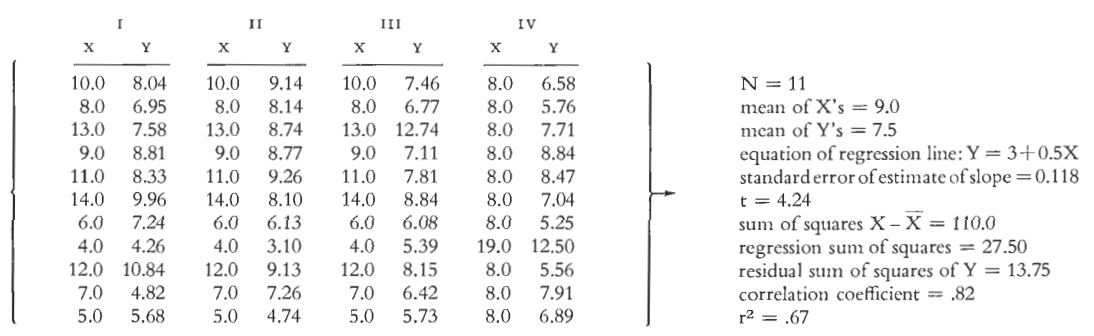
\includegraphics[width=0.80\linewidth]{images/TufteExample0.png}\\
   (a)\\
   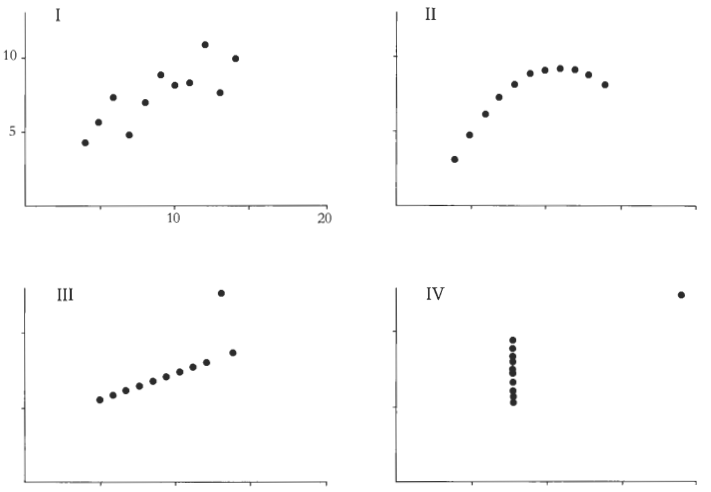
\includegraphics[width=0.80\linewidth]{images/TufteExample1.png}\\
   (b)
   \caption[Tufte example for pattern recognition]{An example for pattern recognition taken from \cite{Tufte}. (a) Tabular data with a statistical analysis. (b) Visualization of the data. As we can see, we can find more relationships from data using information visualization.}
   \label{fig:TufteExample}
\end{figure}

Abstract data used in information visualization can be both numerical and non-numerical. However if the data is generated by scientific inquiry we say we have \textbf{scientific visualization}. Another definition can be taken from \cite{Munzner}:
\begin{definition}[Information visualization]
It's infovis [information visualization] when the spatial representation is chosen, and it's scivis [scientific visualization] when the spatial representation is given                                                                                                                                                                                                                                                                                                                             \end{definition}

As shown, information visualization and scientific visualization are quite similar sciences although they are not identical. In fact, the former represents entities with no direct physical correspondence and devises a physical metaphor; the latter represents something physical or geometric. As this work is based on scientific visualization, and in particular on the representation of biological models, we will focus only on it.\\

Scientific visualization is an interdisciplinary branch of science. According to~\cite{Friendly} it is:
\begin{quotation}
"primarily concerned with the visualization of three-dimensional phenomena (architectural, meteorological, medical, biological, etc.), where the emphasis is on realistic renderings of volumes, surfaces, illumination sources, and so forth, perhaps with a dynamic (time) component".
\end{quotation}
As established from this definition, it can be considered a subset of computer graphics because of the several concepts taken from that discipline.\\

Now we can wonder why this science is so important. In effect, in these years we have observed continuous improvements in scientific fields. In particular computer science may have aided this progress because it permits to simply process data from other sciences, automating processes in a way it was not possible in the past centuries. Moreover, the enormous improvements of technologies, provoked the increase of data originated by experiments and simulations; computer science (and in particular scientific visualization) has valid methods for mastering problems arising from their volume.\\

In the next part of this chapter, we will study some interesting characteristics of scientific visualization

\section{Scientific visualization applications}\label{sec11:Applications}
Now we will observe some interesting application of scientific visualization, so that we can understand its importance.

\paragraph{Natural sciences}
Common applications of scientific visualization for the natural sciences are:
\begin{itemize}
 \item Rendering of molecules
 \item Visualization of gravitational waves and other physical phenomena of interest
 \item Study of fluids
\end{itemize}

\begin{figure}[htb] %  figure placement: here, top, bottom
   \centering
   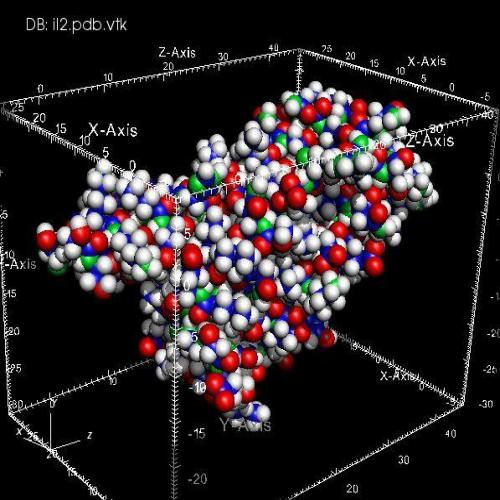
\includegraphics[width=0.30\linewidth]{images/Molecular_rendering.jpg}\hfill
   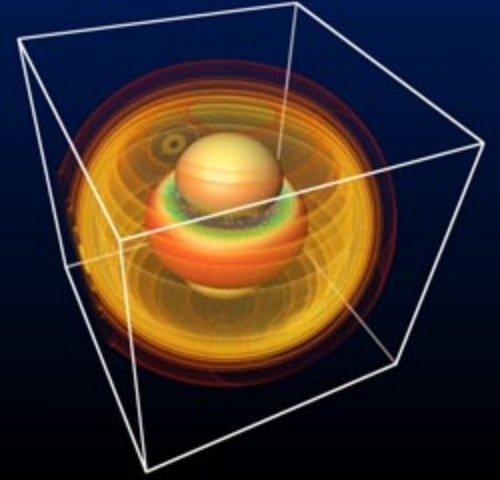
\includegraphics[width=0.30\linewidth]{images/Gravitywaves.JPG}\hfill
   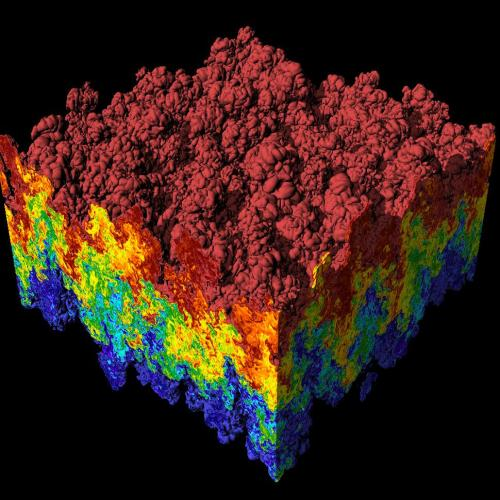
\includegraphics[width=0.30\linewidth]{images/Rayleigh-Taylor_instability.jpg}\hfill\\
   \caption[Examples of scientific visualization applications in natural sciences]{Examples of scientific visualization applications in natural sciences. (a) "Molecular rendering" by UCRL-WEB. (b) "Gravitywaves" by The Globus software creators Ian Foster, Carl Kesselman and Steve Tuecke. (c) "Rayleigh-Taylor instability" by Lawrence Livermore National Laboratory. All images were taken from Wikipedia}
   \label{fig:NaturalSciencesApp}
\end{figure}

\paragraph{Geography}
Common scientific visualization applications for the natural sciences are:
\begin{itemize}
 \item Rendering of terrains
 \item Simulations of atmospheric Anomalies
 \item Climate visualization
\end{itemize}

\begin{figure}[htb] %  figure placement: here, top, bottom
   \centering
   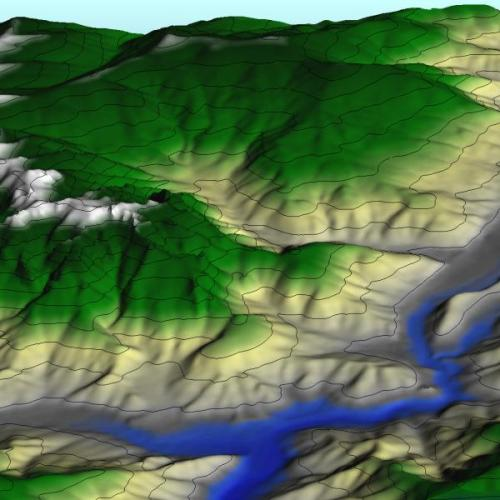
\includegraphics[width=0.30\linewidth]{images/Terrain_rendering.jpg}\hfill
   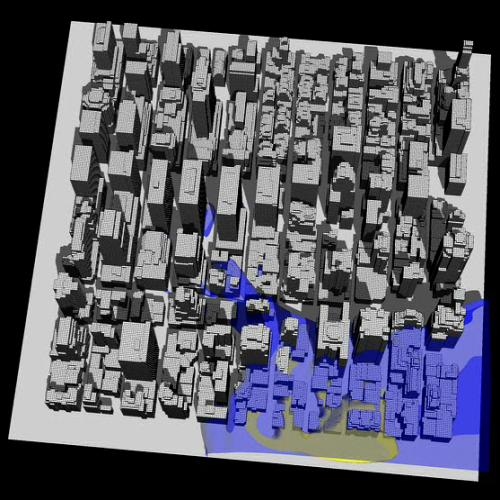
\includegraphics[width=0.30\linewidth]{images/Atmospheric_Anomaly_in_Times_Square.jpg}\hfill
   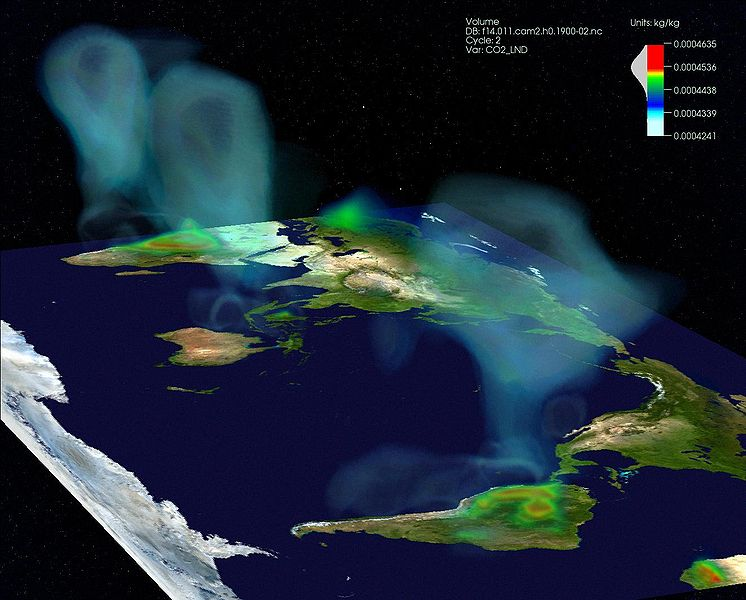
\includegraphics[width=0.30\linewidth]{images/Climate_visualization.jpg}\hfill\\
   \caption[Examples of scientific visualization application in geography]{Examples of scientific visualization application in geography. (a) "Terrain rendering" by UCRL (b) "Atmospheric Anomaly in Times Square" by UCRL and Andrew Wissink Ph.D., LLNL. (c) "Climate visualization" by UCRL and Forrest Hoffman and Jamison Daniel of Oak Ridge National Laboratory. All images were taken from Wikipedia}
   \label{fig:GeographyApp}
\end{figure}

\paragraph{Applied sciences}
Common scientific visualization applications for the natural sciences are:
\begin{itemize}
 \item Visualization of medical images (some techniques will be studied in Chapter~\ref{Chapter13})
 \item Studies on materials
\end{itemize}

\begin{figure}[htb] %  figure placement: here, top, bottom
   \centering
   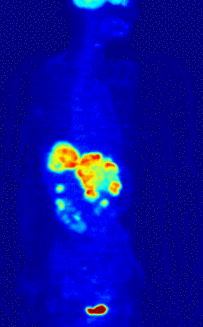
\includegraphics[width=0.30\linewidth]{images/PET-MIPS.png}\hfill
   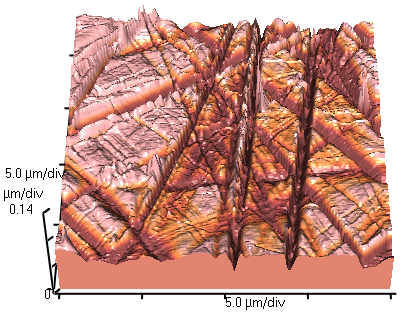
\includegraphics[width=0.45\linewidth]{images/AFMimageRoughGlass.png}
   \caption[Examples of scientific visualization applications in applied sciences]{Examples of scientific visualization applications in applied sciences. (a) "Maximum intensity projection (MIP) of a whole body PET scan" by Jens Maus. (b) "Atomic force microscope topographical scan of a glass surface" by Chych.  All images were taken from Wikipedia}
   \label{fig:AppliedSciencesApp}
\end{figure}

